% To familiarize yourself with this template, the body contains
% some examples of its use.  Look them over.  Then you can
% run LaTeX on this file.  After you have LaTeXed this file then
% you can look over the result either by printing it out with
% dvips or using xdvi.
%

\documentclass[twoside]{article}
%\usepackage{soul}
\usepackage{./lecnotes_macros}


\begin{document}
%FILL IN THE RIGHT INFO.
%\lecture{**LECTURE-NUMBER**}{**DATE**}{**LECTURERS**}{**SCRIBE**}
\lecture{3}{22 January 2025}{Maria Francis and M. V. Panduranga Rao}{Gautam Singh}
%\footnotetext{These notes are partially based on those of Nigel Mansell.}

%All figures are to be placed in a separate folder named ``images''

% **** YOUR NOTES GO HERE:

\section{Cryptanalysis of DES Reduced to 8 Rounds}
DES reduced to 8 rounds uses a 5-round characteristic with probability 
approximately \(\frac{1}{10486}\) as shown in \autoref{fig:des-8-char}.

\begin{figure}[!ht]
    \centering
    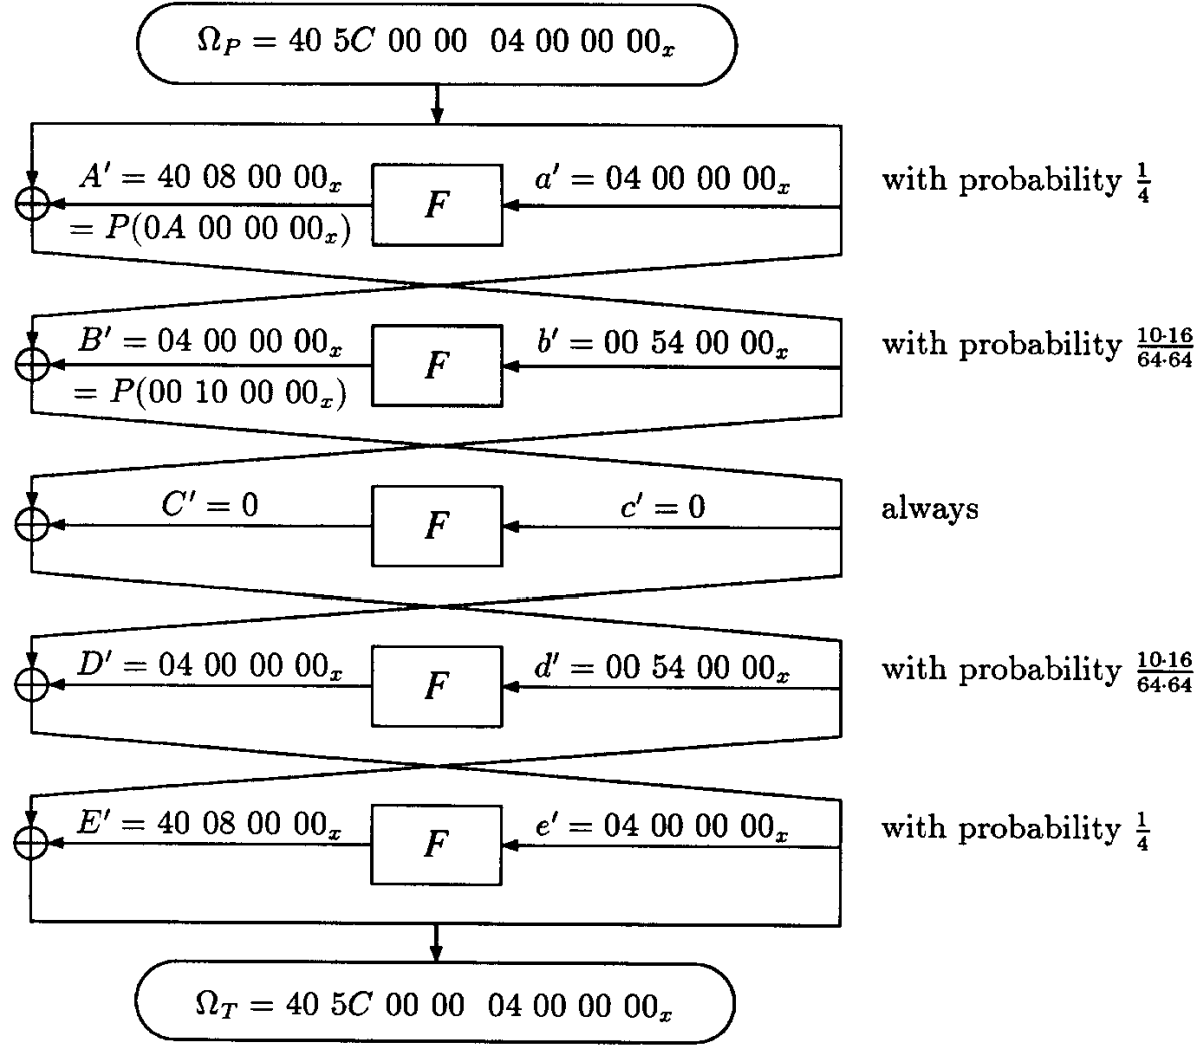
\includegraphics[width=0.5\textwidth]{images/des_8round_char.png}
    \caption{5 round characteristic used to cryptanalyze DES reduced to 8 rounds.}
    \label{fig:des-8-char}
\end{figure}

From the characteristic, it is evident that
\begin{equation}
    f^\prime = d^\prime \oplus E^\prime = b^\prime \oplus A^\prime = L^\prime = \texttt{40 5C 00 00}.
\end{equation}

Thus, for a right pair, five S boxes S2, S5, \dots, S8 have zero input XORs in
the sixth round. Using
\begin{equation}
    H^\prime = l^\prime \oplus g^\prime = l^\prime \oplus e^\prime \oplus F^\prime
\end{equation}

and the fact that \(h^\prime = r^\prime\), we can count on \(5 \cdot 6 = 30\)
key bits of \(K8\). The signal to noise ratio is \(S/N = \frac{2^{30}}{4^5 \cdot
10486} \approx 100\). However, due to the large memory requirement of \(2^{30}\)
locations, we count on fewer key bits. Further, due to the small probability of
the characteristic, we require many plaintexts, which makes the clique method
slow. Notice that each S box discards 20 \% of wrong pairs. Thus, counting on 24
key bits has \(S/N = \frac{2^{24}}{4^4 \cdot 0.8 \cdot 10486} \approx 7.8\) and
counting on 18 key bits has \(S/N = \frac{2^{18}}{4^3 \cdot 0.8^2 \cdot 10486}
\approx 0.6\).

\subsection{Modifying the Characteristic}
By reducing the number of key bits to count, we can also choose which key bits
are to be counted in order to improve the signal to noise ratio. Notice that

\begin{equation}
    e^\prime = \texttt{04 00 00 00} \rightarrow E^\prime = P\brak{\texttt{0W 00 00 00}} = \texttt{X0 0Y Z0 00}
    \label{eq:des-8-r5-rel}
\end{equation}

where \(W \in \cbrak{0,1,2,3,8,9,A,B},\ X,Z \in \cbrak{0,4},\ Y \in
\cbrak{0,8}\). Hence, we have \(f^\prime = d^\prime \oplus E^\prime = \texttt{X0
5V Z0 00}\) where \(V = Y \oplus 4\). If \(Z = 0\), then necessarily \(E^\prime
= \texttt{40 08 00 00}\) and this happens with probability \(\frac{16}{64}\).
All other combinations involving \(Z = 4\) occur with probability
\(\frac{20}{64}\).

Although we cannot count on \(S5_{Kh}\), one can check \(S5^\prime_{Eh}
\rightarrow S5^\prime_{Oh}\) which is satisfied by approximately 80 \% of the
pairs. Thus, the modified probability of \(e^\prime \rightarrow E^\prime\) is
\(\frac{16}{64} + 0.8\frac{20}{64} = \frac{1}{2}\). This doubles the probability
of the characteristic \(\Omega_P\) to \(\frac{1}{5243}\) and consequently
doubles the \(S/N\) for counting on 24 bits and 18 bits of \(K8\) to \(15.6\)
and \(1.2\) respectively.

Counting on 24 subkey bits, we only require about five right pairs due to the
high \(S/N\). This gives us approximately 25000 plaintext pairs. For 18 subkey
bits, we need about 150000 pairs. The average count per key is \(\frac{150000
\times 4^3 \times 0.8^2}{2^18} = 24\) and the right key is counted an additional
\(\frac{150000}{5243} = 29\) times, giving a total count of \(24 + 29 = 53\) for
the right key.

However, this finds us 18 subkey bits, say entering S6, S7 and S8. To find the
other 12 subkey bits entering S2 and S5 in the eighth round, we filter the pairs
that correspond to the subkey values in S6, S7 and S8. The expected number of
pairs is then 53. Counting on the remaining 12 bits using these right pairs
leads to a higher \(S/N\) which can filter more pairs.

Now, using the known 30 subkey bits of \(K8\), we can find the dependence of the
bits of \(S_{Eg}\) and \(S_{Kg}\) on \(K8\), shown in \autoref{fig:des-8rd-dep}.

\begin{figure}[!ht]
    \centering
    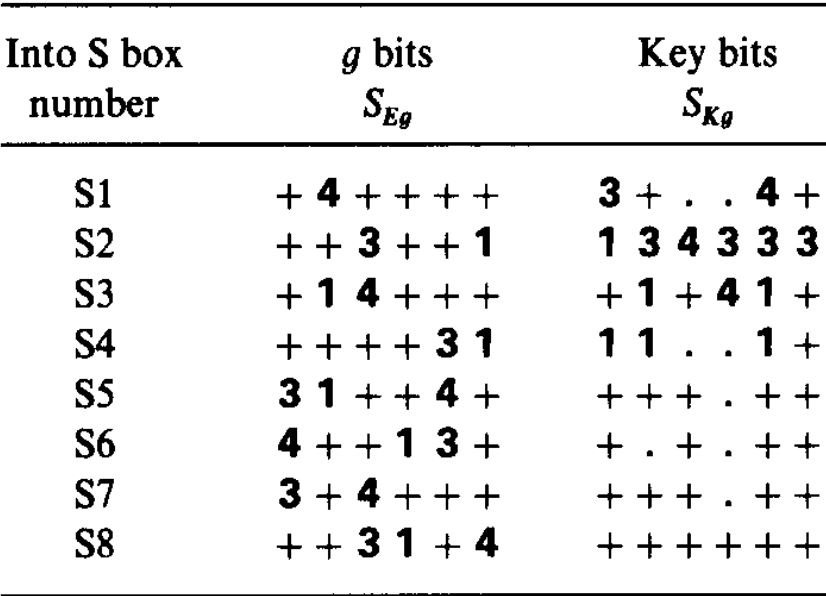
\includegraphics[width=0.5\linewidth]{images/des_8round_dep.png}
    \caption{Dependence of bits at the seventh round on those of the eighth round. `+' indicates dependence on known key bits, `.' indicates dependence on other key bits and a number indicates dependence on unknown key bits that enter the corresponding S box in the eighth round.}
    \label{fig:des-8rd-dep}
\end{figure}

By checking using the formula \(G^\prime = f^\prime \oplus h^\prime\) for S2, S3
and S8, we can brute force the remaining 18 key bits of \(K8\). This equation
holds for all filtered pairs. A faster way is to count on the 12 bits entering
S1 and S4 in the eighth round, since they compute \(S3^\prime_{Og}\). After
further filtration, we count on the remaining 6 subkey bits to get \(K8\)
completely. Brute-force on the remaining 8 bits unused in \(K8\) will give us
the master key.

\subsection{Speeding Up the Attack}
Post every step of filtration, wrong pairs can be discarded. Counting on 24 bits
will reduce the 25000 pairs to \(25000 \times 0.8^5 \approx 7500\) pairs.
However, this is not so good for counting on 18 bits. The authors devised
another criterion based on a weighting function and a threshold. This weighting
function is the product of the number of possible keys of each of the five
countable S boxes. A right pair would suggest more possible keys than a wrong
pair at an S box, thus a carefully chosen threshold can discard the wrong pairs.
Experimentally, setting a threshold of 8192 discards about 97 \% of right pairs.
This reduces the number of pairs analyzed from 150000 to 7500 and greatly speeds
up the attack.

\subsection{Enhanced Characteristics}
The authors list two ways to boost the probability of characteristics and
enhance signal-to-noise ratio.

\begin{enumerate}
    \item By exploiting possible input and output XORs in S boxes, we can
    eliminate some possibilities. For instance, \autoref{fig:s2-xor-bits} shows
    that for \(08_x \rightarrow A_x\), the bits at positions 2 and 6 are always
    equal. Thus, we can use plaintexts which cause these bits to be equal. We
    can see that both bits equal 0 with probability \(\frac{12}{16}\) and both
    equal 1 with probability \(\frac{4}{16}\). This improves the probability of
    the characteristic to \(\frac{1}{2}\), doubling the \(S/N\).  

    \begin{figure}[!ht]
        \centering
        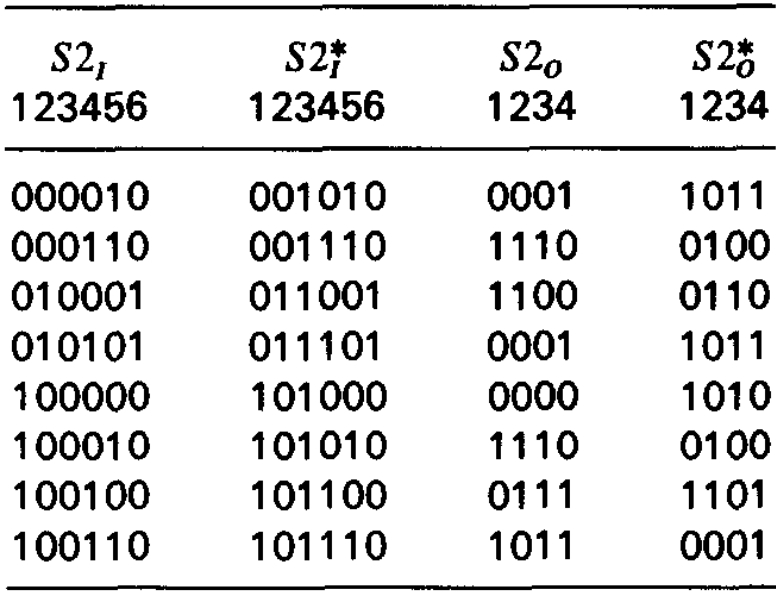
\includegraphics[width=0.5\linewidth]{images/s2_xor_bits.png}
        \caption{Possible instances for \(08_x \rightarrow A_x\) by S2.}
        \label{fig:s2-xor-bits}
    \end{figure}

    \item In case the key bits at those positions are known, then we could
    choose the \(\frac{12}{16}\) case which triples the \(S/N\).
\end{enumerate}

\subsection{Extension to Nine Rounds}
We concatenate the following characteristic with the one in
\autoref{fig:des-8-char} to cryptanalyze DES reduced to 9 rounds.

\begin{figure}[!ht]
    \centering
    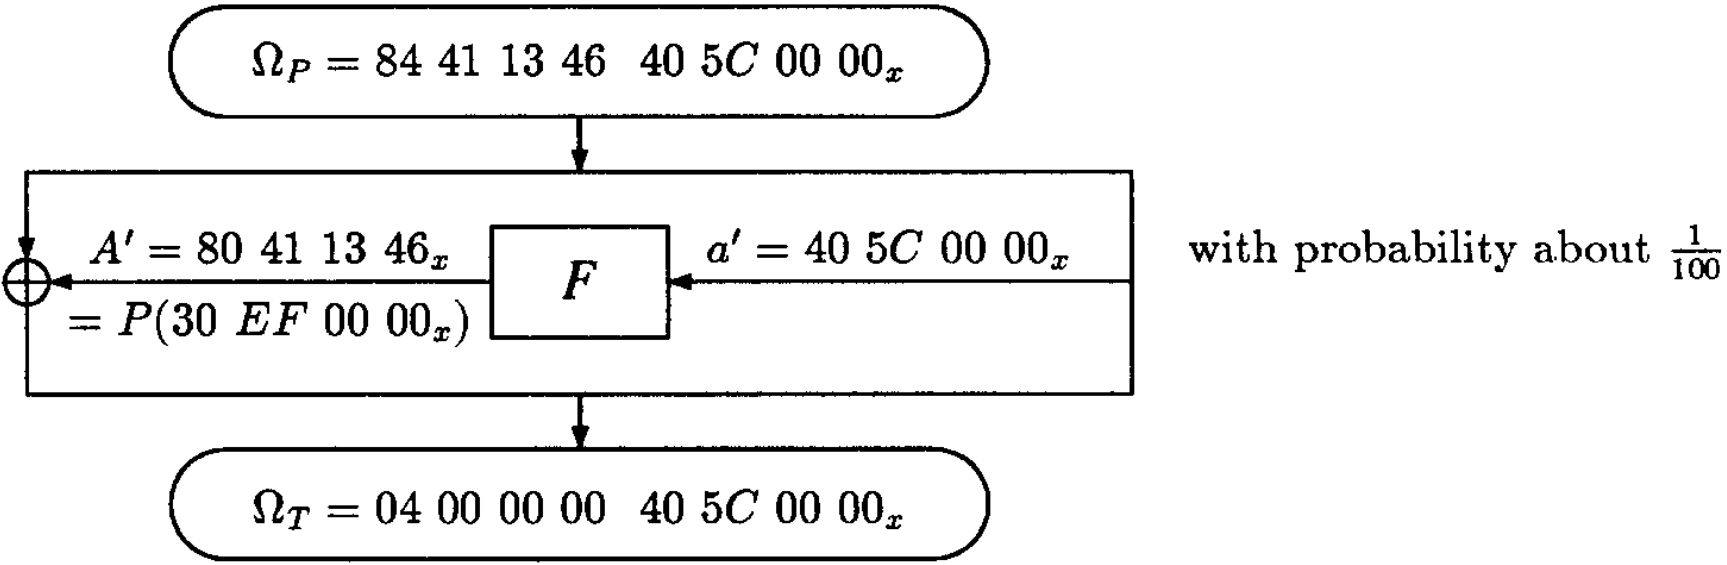
\includegraphics[width=0.5\linewidth]{images/des_9round_char.png}
    \caption{Characteristic to be concatenated to cryptanalyze DES reduced to 9 rounds.}
    \label{fig:des-9-char}
\end{figure}

The entire six-round characteristic has probability \(\approx 10^{-6}\). Thus,
counting on 30 subkey bits gives \(S/N = \frac{2^{30}}{4^5 \cdot 10^6} \approx
1\). After finding these 30 subkey bits, a similar process is followed by
exploiting the relations between bits in the eighth and ninth round to get the
other 18 bits of \(K9\). Due to the low \(S/N\), we require about 30 million
pairs.

\section{DES with an Arbitrary Number of Rounds}

\subsection{Iterative Characteristics}
To cryptanalyze DES reduced to an aribitrary number of rounds, we make use of an
\emph{iterative} characteristic. Such a characteristic can be concatenated with
itself to generate longer characteristics. An iterative characteristic is shown
in \autoref{fig:des-iter-char}.

\begin{figure}[!ht]
    \centering
    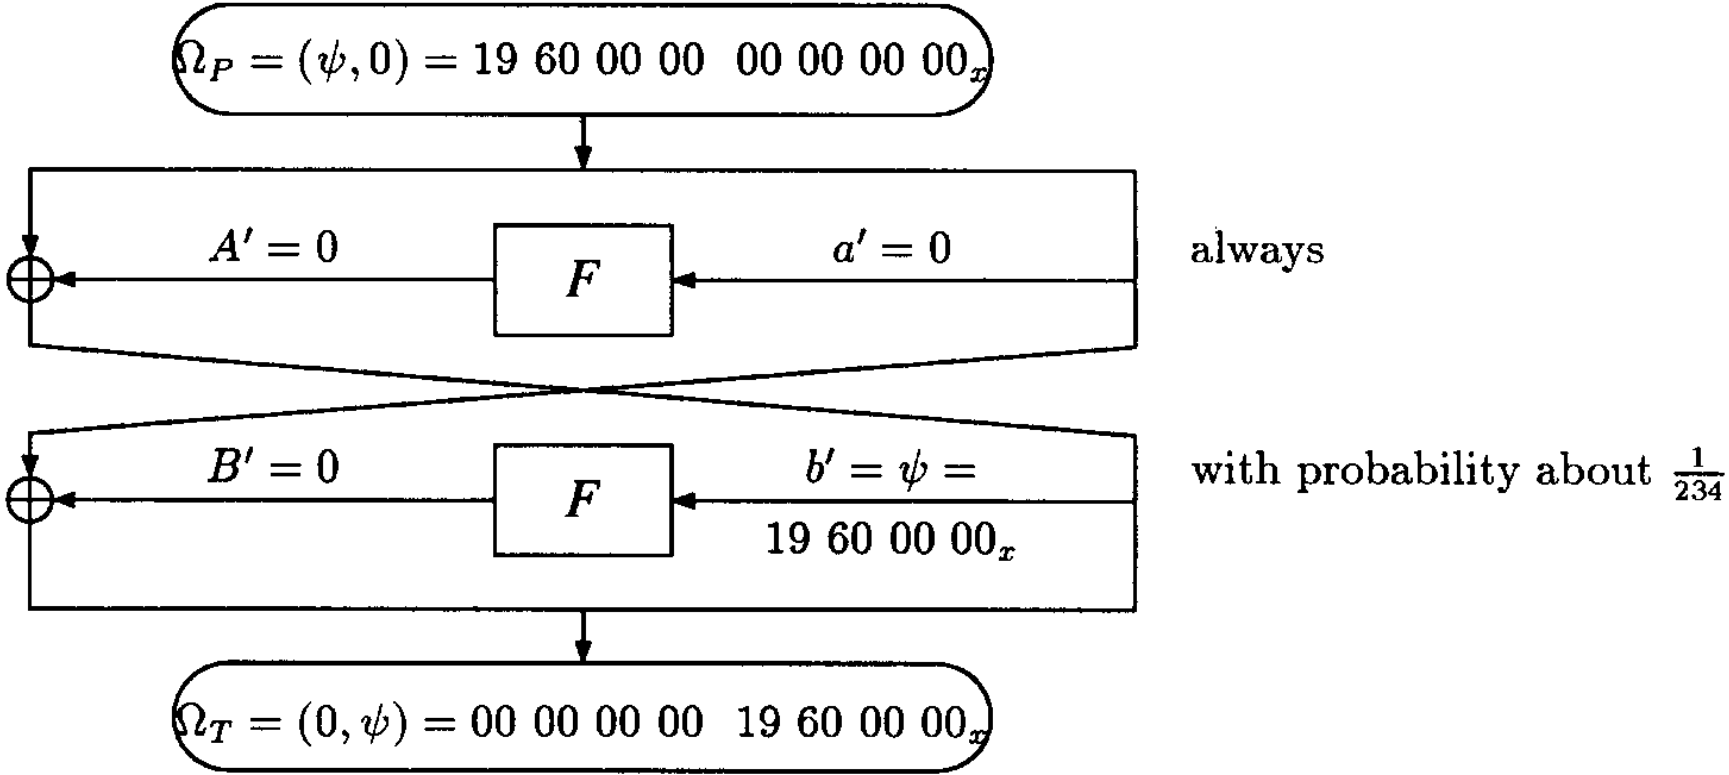
\includegraphics[width=0.5\linewidth]{images/des_iter_char.png}
    \caption{Iterative characteristic with probability \(\frac{1}{234}\). Another value for \(\psi\) could be \texttt{1B 60 00 00}.}
    \label{fig:des-iter-char}
\end{figure}

This iterative characteristic has probability \(\approx 2^{-56}\) when extended
to 15 rounds. Thus, using this characteristic to cryptanalyze the entire DES
performs worse than exhaustive search.

Depending on the additional number of rounds in the cryptosystem that are
outside of the characteristic, we can categorize attacks into four types. In
most cases these additional rounds are the last rounds of the cryptosystem.

\subsection{3R-Attacks}
These have 3 additional rounds in the cryptosystem. DES reduced to 4, 8 or 9
rounds can be cryptanalyzed with this kind of attack. For DES reduced to 8
rounds, using the iterative characteristic with probability about
\(\frac{1}{234^2} = \frac{1}{55000}\), counting on 24 key bits gives \(S/N =
\frac{2^{24}}{4^4 \cdot 0.8 \cdot 55000} \approx 1.5\) and counting on 30 key
bits gives \(S/N = \frac{2^{30}}{4^5 \cdot 55000} \approx 19\), reducing the
number of pairs to \(\brak{1 - 0.8^5} = 67 \%\) of the original.

For a fixed cryptosystem, 3R attacks have shorter characteristics with better
probability, thus they are the most useful.

\subsection{2R-Attacks}
These have 2 additional rounds in the cryptosystem. To boost the \(S/N\),
possibility checks can be performed for all previous round S boxes, that is,
predicting whether an input-output XOR pair is possible.

For example, in DES reduced to 9 rounds, we can use the iterative characteristic
with probability \(2^{-24}\) for seven rounds. The iterative characteristic
gives

\begin{align}
    h^\prime &= \psi \rightarrow H^\prime = i^\prime \oplus g^\prime = r^\prime \label{eq:des-9rd-h} \\
    i^\prime &= r^\prime \rightarrow I^\prime = h^\prime \oplus l^\prime = \psi \oplus l^\prime \label{eq:des-9rd-i}
\end{align}

For \(h^\prime \rightarrow H^\prime\), five S boxes have zero input XOR. A wrong
pair can pass through this S box with probability \(\frac{1}{16}\). For the
other three S boxes this probability is \(0.8\). Hence, counting on all 48 bits
of \(K9\) has \(S/N = \frac{2^{48} \cdot 2^{-24}}{4^8 \cdot 0.8^3 \cdot 16^{-5}}
\approx 2^{29}\). Counting on 18 bits has \(S/N = \frac{2^{18} \cdot
2^{-24}}{4^3 \cdot 0.8^5 \cdot 0.8^3 \cdot 16^{-5}} \approx 2^{11}\). Counting
on just 6 key bits has \(S/N = \frac{2^6 \cdot 2^{-24}}{4 \cdot 0.8^7 \cdot
0.8^3 \cdot 16^{-5}} \approx 10\). By checking with the previous round S boxes,
we are left with \(0.8^3 \cdot 16^{-5} = 2^{-24}\) wrong pairs. Since the
characteristic has probability \(2^{-24}\), we require \(2^{26}\) pairs for
cryptanalysis.

Similar analyses can be carried out for DES reduced to 11, 13 and 15 rounds.
However, more plaintext pairs are required for cryptanalysis which makes the
attacks unrealistic.

\subsection{1R-Attacks}
These have only one additional round in the cryptosystem. Here, we can only
verify the value of \(r^\prime\) and perform possibility checks on the S boxes
of the last round only. The input XOR to the last round is constant, thus we
cannot single out a subkey value for each S box. Instead, we have to
exhaustively search these key values (which are reduced in number due to the
input-output XOR pair).

For example, DES reduced to 10 rounds can be broken with the 9 round
characteristic where

\begin{align}
    i^\prime &= 0 \rightarrow I^\prime = 0 \label{eq:des-10rd-i} \\
    j^\prime &= \psi \rightarrow J^\prime = l^\prime \oplus i^\prime = l^\prime \label{eq:des-10rd-j}
\end{align}

Right pairs satisfy \(r^\prime = \psi\) and the 20 bits in \(l^\prime\) going
out of S4, \dots, S8 are zero. This holds for \(2^{-32} \cdot (2^{-4})^5 =
2^{-52}\) of the wrong pairs. For the other three S boxes, we count on the 18
key bits to get \(S/N = \frac{2^{18} \cdot 2^{-32}}{4^3 \cdot 2^{-52}} =
2^{32}\). Thus, we require \(2^{34}\) pairs.

\end{document}
